
\chapter{Process description and control}

\subsection{What is a process?}

A process consists of program code and associated data plus a process control block. For a single-processor computer, at any given time, at
most one process is executing and that process is in the running state.\\

Each control block contains data about the process to be able to uniquely identify them:

• Identifier: A unique identifier associated with this process, to distinguish it
from all other processes.\\
• State: If the process is currently executing,it is in the running state.\\
• Priority: Priority level relative to other processes.\\
• Program counter: The address of the next instruction in the program to be
executed.\\
• Memory pointers: Includes pointers to the program code and data associated
with this process,plus any memory blocks shared with other processes.\\
• Context data: These are data that are present in registers in the processor
while the process is executing.\\
• I/O status information: Includes outstanding I/O requests,I/O devices (e.g.,tape
drives) assigned to this process,a list of files in use by the process,and so on.\\
• Accounting information: May include the amount of processor time and clock
time used,time limits,account numbers,and so on.\\

\\
\\
\begin{figure}
\centering
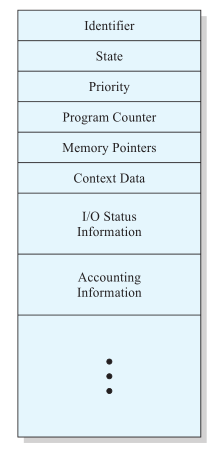
\includegraphics{img/simplifiedcontrolblock.PNG}
\caption{Simplified Control Block}
\label{fig:simpblock}
\end{figure}


\subsection{Process creation}
When a new process is to be added to those currently being
managed,the OS builds the data structures that are used to manage the process and
allocates address space in main memory to the process. 

Reasons for process creation:\
• New batch job: The OS is provided with a batch job control stream,usually on tape or
disk.When the OS is prepared to take on new work,it will read the
next sequence of job control commands.\\
• Interactive logon: A user at a terminal logs on to the system.\\
• Created by OS to provide a service: The OS can create a process to perform a function on behalf of a user
program,without the user having to wait (e.g.,a process to control
printing).\\
• Spawned by existing process: For purposes of modularity or to exploit parallelism,a user program
can dictate the creation of a number of processes.\\


\\
\\

\subsection{Process termination}

Reasons for process termination:\

• Normal completion: The process executes an OS service call to indicate that it has completed
running.\\
• Time limit exceeded: The process has run longer than the specified total time limit.There are a
number of possibilities for the type of time that is measured.These include
total elapsed time (“wall clock time”),amount of time spent executing,and,
in the case of an interactive process,the amount of time since the user last
provided any input.\\
• Memory unavailable: The process requires more memory than the system can provide.\\
• Bounds violation: The process tries to access a memory location that it is not allowed to access.\
• Protection error: The process attempts to use a resource such as a file that it is not allowed
to use,or it tries to use it in an improper fashion,such as writing to a read-
only file.\\
• Arithmetic error: The process tries a prohibited computation,such as division by zero,or tries
to store numbers larger than the hardware can accommodate.\\
• Time overrun: The process has waited longer than a specified maximum for a certain event
to occur.\\
• I/O failure: An error occurs during input or output,such as inability to find a file,failure
to read or write after a specified maximum number of tries (when,for exam-
ple,a defective area is encountered on a tape),or invalid operation (such as
reading from the line printer).\\
• Invalid instruction: The process attempts to execute a nonexistent instruction (often a result of
branching into a data area and attempting to execute the data).\\
• Privileged instruction: The process attempts to use an instruction reserved for the operating system.\\
• Data misuse: A piece of data is of the wrong type or is not initialized.\\
• Operator or OS intervention: For some reason,the operator or the operating system has terminated the
process (for example,if a deadlock exists).\\
• Parent termination: When a parent terminates,the operating system may automatically termi-
nate all of the offspring of that parent.\\
• Parent request: A parent process typically has the authority to terminate any of its offspring.\\


\subsection{Process states}

\begin{figure}
\centering
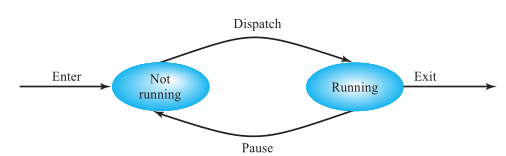
\includegraphics{img/twostate.PNG}
\caption{Two state process}
\label{fig:simpblock}
\end{figure}

\begin{figure}
\centering
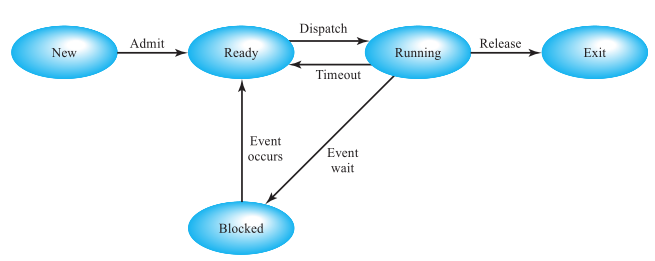
\includegraphics{img/fivestate.PNG}
\caption{Five state process}
\label{fig:simpblock}
\end{figure}

